\par System zarządzania jest narzędziem umożliwiającym planowanie, organizowanie i kontrolowanie postępów w pracy nad wieloma projektami i zadaniami. Każdy użytkownik może mieć różne uprawnienia przy różnych projektach, a manager i administrator mają pełną kontrolę nad swoimi zasobami.
			\par Utworzenie tego narzędzia w formie aplikacji internetowej, obsługiwanej przez dedykowany serwer umożliwia użytkownikom swobodny dostęp do informacji z dowolnego miejsca, o dowolnym czasie. Analogicznie osoby do tego uprawnione, w każdym momencie mogą zarządzać projektami i wprowadzać zmiany.
			\par System daje możliwość organizacji nieskończonej ilości niezależnych projektów. Przy każdym projekcie możemy zdefiniować typy zagadnień jak i moduły: Śledzenie zagadnień, Śledzenie czasu, Komunikaty, Dokumenty, Pliki, Wiki, Fora, Repozytorium, Diagram Gantta, Kalendarz oraz wiele innych.
			\par Systemy zarządzania dzielimy na dwie kategorie. Pierwszą kategorią są systemy zarządzania relacji z klientami nazywane z ang. CRM (Client Relation Managment), drugą systemy zarządzania zasobami przedsiębiorstwa nazywane z ang. ERP (Enterprise Resource Planning).
			\par Wybrany system zarządzania to "redmine" wraz z modułami CRM i Commerce. Jest to aplikacja internetowa napisana w języku ruby. Współpracuje ona z bazą danych PostgreSQL i jest często wykorzystywana do zarządzania projektami różnego typu. W tym wypadku możemy potraktować każdą sprzedaż jako osobny projekt składający się z kilku procesów.

				\par System zarządzania składa się z następujących elementów zapewniających kontrolę w różnych obszarach prowadzenia działalności.
		
	\begin{description}
		\item[\textbf{Główna}] - przenosi użytkownika na stronę główną,
	
		\item[\textbf{Moja strona}] - przenosi użytkownika do strony, która służy do nawigacji po całej aplikacji, domyślnie są tu widoczne najnowsze przypisane do użytkownika zagadnienia, oraz najnowsze zgłoszone przez niego zagadnienia. Stronę tę można personalizować klikając przycisk "Personalizuj stronę".
					
		\item[\textbf{Projekty}] - przenosi na stronę, gdzie prezentowane są użytkownikowi wszystkie projekty w jakich bierze udział. Projekty, których użytkownik jest kierownikiem oznaczone są gwiazdką. Strona ta umożliwia również przeglądanie wszystkich przypisanych do użytkownika zagadnień (niezależnie od projektu), przeprowadzonego przez niego czasu oraz przejrzenie jego ogólnej aktywności we wszystkich projektach,
					
		\item[\textbf{Kontakty}] - przenosi na kartę, gdzie widoczne są dodane już kontakty. Przy odpowiednich uprawnieniach w kolejnym kroku można edytować lub dodawać kontakty.
					
		\item[\textbf{Faktury}] - wtyczka ta pomaga obsługiwać faktury, upraszcza pracę między innymi poprzez umożliwienie bezpośredniego eksportowania do formatu PDF, wydrukowania bądź wysłania faktury do klienta. Znajdują się tutaj filtry do sprawnej nawigacji po historii wystawianych faktur jak i funkcja sortowania. Można również dodawać faktury, których wystawienie jest dopiero planowane.
					
		\item[\textbf{Finanse}] - sekcja ta pozwala na łatwe zarządzanie i kontrolowanie płatności dokonywanych przez firmę bądź klientów poprzez bardzo przejrzysty interfejs. Są tu funkcje filtrowania jak i sortowania wszystkich transakcji dla poprawy nawigacji. Moduł pozwala również na obsługę różnych kont bankowych co pomaga w rozliczeniach przy użyciu rachunków umieszczonych w różnych instytucjach bankowych, oraz pozwala śledzić sytuację finansową firmy.
					
		\item[\textbf{Osoby}] - jest to książka telefoniczna firmy, gdzie znajdują wszystkie kontakty, z którymi firma nawiązała jakieś interakcje
					
		\item[\textbf{Produkty}] - tutaj zawarte są wszystkie produkty, które firma miała w ofercie. Zarówno te aktualnie znajdujące się  w ofercie jak i te nieaktywne
					
		\item[\textbf{Zamówienia}] - w tej karcie są wszystkie zamówienia kiedykolwiek podjęte przez firmę
					
		\item[\textbf{Administracja}] - na tej stronie możemy zarządzać systemem. Oprócz wyznaczania uprawnień różnym użytkownikom, możemy też między innymi zmieniać wygląd aplikacji i tym podobne
					
		\item[\textbf{Pomoc}] - tutaj znajdziemy wszystkie informacje, dzięki którym będziemy mogli sprawnie obsługiwać system
	\end{description}
	
	\subsubsection{Projekty} 
		\par Po wybraniu jednego z widocznych projektów (czyli takich, których jesteśmy członkiem lub będących projektem publicznym) dostępne staje się dodatkowe menu. Dostępne tutaj opcje to:
	
		\begin{description}
			\item[\textbf{Przegląd}] - strona prezentuje ogólne informacje o projekcie, takie jak strona domowa, pod projekty, liczbę i rodzaj zagadnień czy listę i grupy uczestników projektu. Strona ta pozwala również kierownikowi projektu na jego zamknięcie i utworzenie pod projektu.
	
			\item[\textbf{Aktywność}] - strona prezentuje wszystkie zdarzenia, jakie miały miejsce w projekcie.
	
			\item[\textbf{Zagadnienia}] - strona pozwala na przeglądanie zagadnień przypisanych do projektu i jego pod projektów, możliwe jest ich filtrowanie czy też grupowa zmiana statusu.
	
			\item[\textbf{Gantt}] - strona umożliwia przeglądanie stanu zaawansowania realizacji zagadnień w postaci wykresu Gantt'a. Do poprawnego działania wymaga dokładnego uzupełnienia danych zagadnienia, w szczególności dat.
	
			\item[\textbf{Kalendarz}] - strona umożliwia przeglądanie stanu zaawansowania realizacji zagadnień w postaci kalendarza. Do poprawnego działania wymaga dokładnego uzupełnienia danych zagadnienia, w szczególności dat.
	
			\item[\textbf{Komunikaty}] - strona umożliwia przeglądanie i definiowanie komunikatów dla osób zainteresowanych projektem.
	
			\item[\textbf{Dokumenty}] - strona umożliwia przeglądanie i zarządzanie dokumentami.
	
			\item[\textbf{Wiki}] - strona umożliwia przeglądanie i edycje stron Wiki czyli dokumentacji firmy. Jest to miejsce, w którym można opisać firmowe procedury.
	
			\item[\textbf{Pliki}] - strona umożliwia przeglądanie i zarządzanie udostępnianymi plikami, dzięki tej funkcjonalności można w bezpieczny sposób katalogować, przechowywać i udostępniać pliki. 
	
			\item[\textbf{Ustawienia}] - strona umożliwiająca zmianę ustawień projektu, aktywację/dezaktywację modułów itp.
						
			\item[\textbf{Kontakty}] - strona ta zawiera listę wprowadzonych do systemu kontaktów. Pozwala również na zarządzanie listą kontaktów.

			\item[\textbf{Faktury}] - strona wyświetlająca listę faktur. Daje ona możliwości wystawienia i planowania faktur, oraz ich eksportu do formatu PDF.

			\item[\textbf{Finanse}] - znajduje się tu rejestr operacji finansowych. Są dokonywane na kontach, które można zdefiniować w tym module.

			\item[\textbf{Produkty}] - lista produktów będących w sprzedaży. Można tu dodać produkty wraz z opisem, zdjęciami i opcjami.

			\item[\textbf{Zamówienia}] - na tej stronie znajdują się wszystkie zamówienia zrealizowane przez firmę, umożliwia to wyliczenie obrotu w zależności od kontrahenta.

			\item[\textbf{Periodic Task}] - strona ta odpowiada za konfigurację powtarzających się w czasie zdarzeń. Użytkownik może dodawać zdarzenia wraz ze zdefiniowanym okresem powtarzania. 

		\end{description}
				 
		\subsubsection{Faktury}
			\par Dodawanie faktur działa w sposób intuicyjny, wszystkie dane do faktury wpisywane są w oddzielnych polach, oprócz tego można w przypadku współpracy z zagranicznymi klientami określić wersję językową faktury, formularz jest na tyle szczegółowy, że nawet znalazło się w nim miejsce na uwzględnienie rabatu dla kontrahenta. Na podstawie wszystkich wpisanych danych, system generuje fakturę w formacie PDF, którą można od razu wydrukować bądź wysłać do klienta.
					
		\subsubsection{Finanse}
			\par W tej sekcji możemy określić typ dokumentowanej operacji, umieścić wszystkie dane jej dotyczące, między innymi jej wartość, dodać opis, a jeżeli jest to konieczne, również załączniki potrzebne do dokumentacji. Oprócz tego możemy dodać konto, na którym po zapisaniu będzie można wykonywać operacje finansowe.
					
		\subsubsection{Przykładowe funkcjonalności}	
					
			\begin{figure}[H]
				\centering
				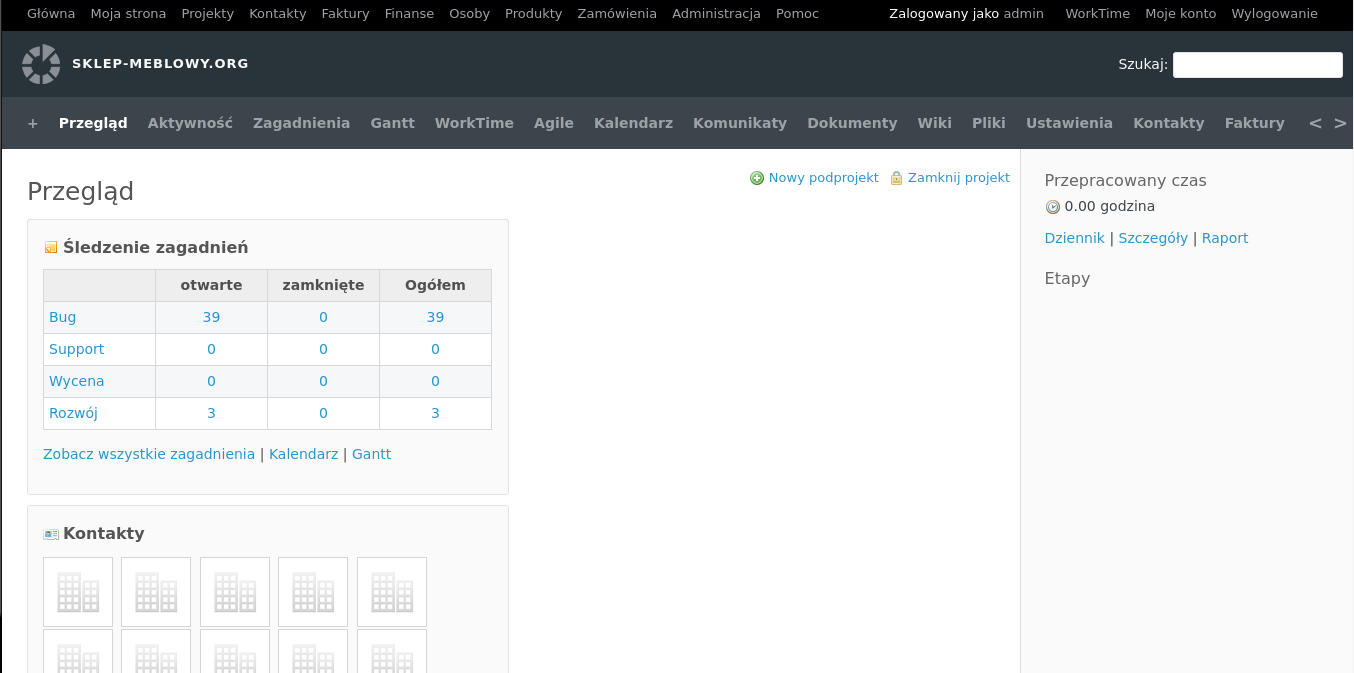
\includegraphics[scale=0.40]{crm_main}
				\caption{Strona główna}
			\end{figure}
					
			\begin{figure}[H]
				\centering
				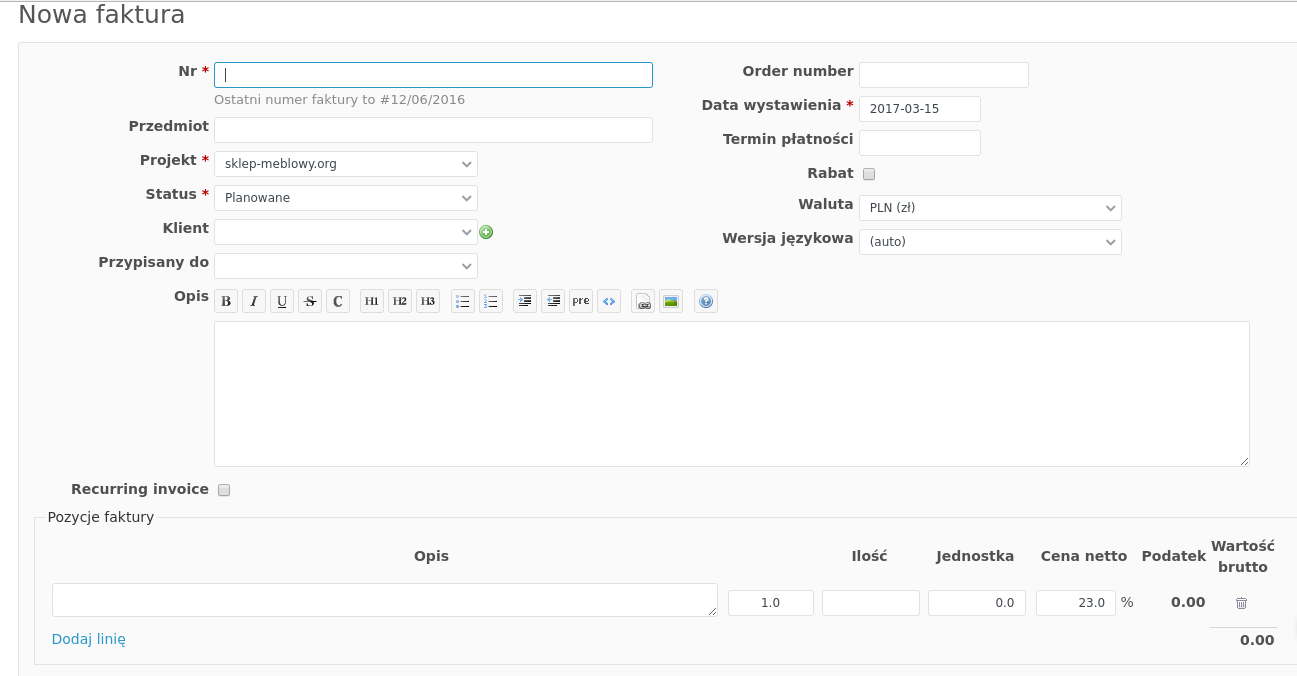
\includegraphics[scale=0.60]{invoice}
				\caption{Fragment formularza służącego do wystawienia nowej faktury}
			\end{figure}
					
			\begin{figure}[H]
				\centering
				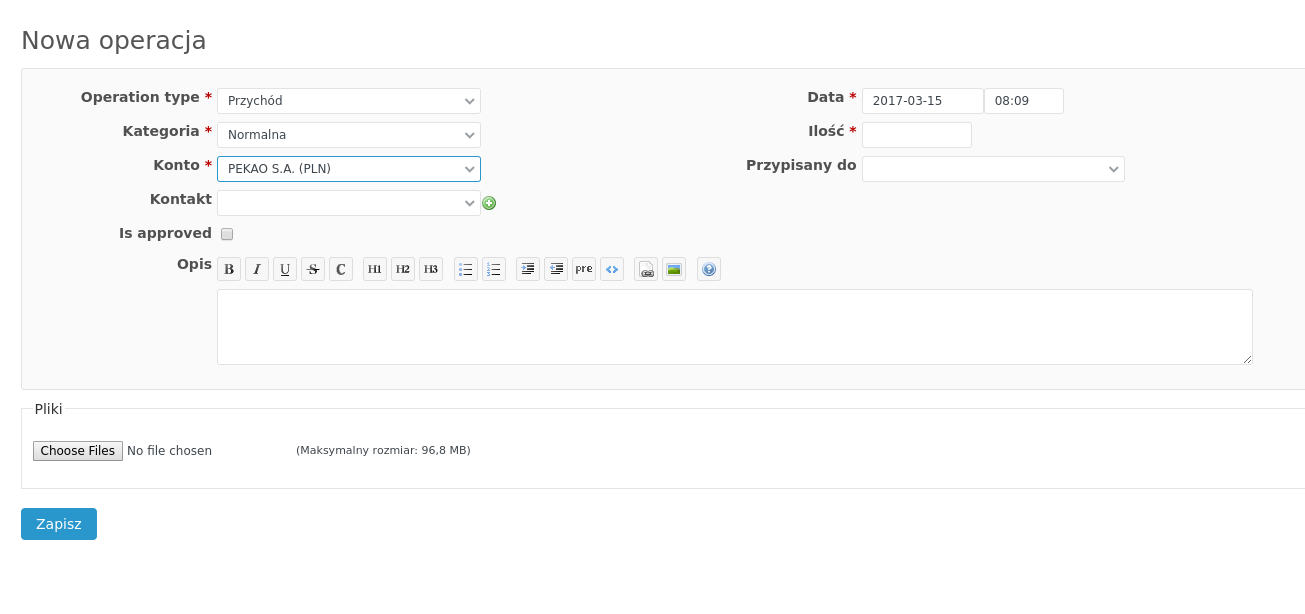
\includegraphics[scale=0.60]{finance}
				\caption{Fragment formularza nowej operacji finansowej}
			\end{figure}

 
